\documentclass[11pt,a4paper]{report}  
% Aberystwyth MMP Project Report Template for LaTeX
%
% Authors: Neil Taylor (nst@aber.ac.uk) and Dr. Hannah Dee (hmd1@aber.ac.uk) 
%
% This has been adapted from the Leeds Thesis template and the 
% Group Project template for Computer Science in Aberystwyth University.
% 
% All comments and suggestions welcome.
%
% Template designed to be used with pdflatex: it may need alteration to
% run with a different LaTeX engine.
%
% Note - this is offered as a starting point for your work. You are not 
% required to use this template and can choose to create your own document 
% without it.

% This template is suitable for students with an engineering-style project, 
% which will be most students in the department. If your project is a research-oriented 
% project, look at the alternative template.

% To build document on the unix command line, run four commands:
 
% pdflatex mmp-report
% bibtex mmp-report
% pdflatex mmp-report
% pdflatex mmp-report

% you will end up with mmp-report.pdf. Before submitting, add your user ID as a prefix, 
% e.g. abc01-mmp-report.pdf 
\usepackage{StylesAndReferences/mmp-report}

\usepackage{graphicx}
\usepackage{caption}
\usepackage{tabularx}
\usepackage{color}
\usepackage{listings}
\usepackage{ltablex}
\usepackage{hyperref}

% Requires package: color.
\definecolor{mediumgray}{rgb}{0.3, 0.4, 0.4}
\definecolor{mediumblue}{rgb}{0.0, 0.0, 0.8}
\definecolor{forestgreen}{rgb}{0.13, 0.55, 0.13}
\definecolor{darkviolet}{rgb}{0.58, 0.0, 0.83}
\definecolor{royalblue}{rgb}{0.25, 0.41, 0.88}
\definecolor{crimson}{rgb}{0.86, 0.8, 0.24}

\lstdefinelanguage[ECMAScript2015]{JavaScript}[]{JavaScript}{
	morekeywords=[1]{await, async, case, catch, class, const, default, do,
		enum, export, extends, finally, from, implements, import, instanceof,
		let, static, super, switch, throw, try},
	morestring=[b]` % Interpolation strings.
}

\lstdefinestyle{JSES6Base}{
	backgroundcolor=\color{white},
	basicstyle=\ttfamily,
	breakatwhitespace=false,
	breaklines=false,
	captionpos=b,
	columns=fullflexible,
	commentstyle=\color{mediumgray}\upshape,
	emph={},
	emphstyle=\color{crimson},
	extendedchars=true,  % requires inputenc
	fontadjust=true,
	frame=single,
	identifierstyle=\color{black},
	keepspaces=true,
	keywordstyle=\color{mediumblue},
	keywordstyle={[2]\color{darkviolet}},
	keywordstyle={[3]\color{royalblue}},
	numbers=left,
	numbersep=5pt,
	numberstyle=\tiny\color{black},
	rulecolor=\color{black},
	showlines=true,
	showspaces=false,
	showstringspaces=false,
	showtabs=false,
	stringstyle=\color{forestgreen},
	tabsize=2,
	title=\lstname,
	upquote=true  % requires textcomp
}

\lstdefinestyle{JavaScript}{
	language=JavaScript,
	style=JSES6Base
}
\lstdefinestyle{ES6}{
	language=ES6,
	style=JSES6Base
}
\lstalias[]{ES6}[ECMAScript2015]{JavaScript}

\lstdefinelanguage{JavaScript}{
	morekeywords=[1]{break, continue, delete, else, for, function, if, in,
		new, return, this, typeof, var, void, while, with},
	% Literals, primitive types, and reference types.
	morekeywords=[2]{false, null, true, boolean, number, undefined,
		Array, Boolean, Date, Math, Number, String, Object},
	% Built-ins.
	morekeywords=[3]{eval, parseInt, parseFloat, escape, unescape},
	sensitive,
	morecomment=[s]{/*}{*/},
	morecomment=[l]//,
	morecomment=[s]{/**}{*/}, % JavaDoc style comments
	morestring=[b]',
	morestring=[b]"
}[keywords, comments, strings]



% the following packages are used for citations - You only need to include one. 
%
% Use the cite package if you are using the numeric style (e.g. IEEEannot). 
% Use the natbib package if you are using the author-date style (e.g. authordate2annot). 
% Only use one of these and comment out or remove the other one. 
\usepackage{cite}
%\usepackage{natbib}

%%%% Title and Section Colours %%%%
% Modify these values to change the colours used for title, sections and subsections.
% Each value is a range of 0-255 in RGB colourspace.
% Idea courtesy of discussion at 
% https://www.overleaf.com/learn/latex/Using_colours_in_LaTeX
% and
% https://tex.stackexchange.com/questions/75667/change-colour-on-chapter-section-headings-lyx
% 
% If you prefer to have black headers, then comment out the following lines
\definecolor{mmpTitle}{RGB}{10, 85, 145}
\definecolor{mmpSection}{RGB}{10,85,155}
\definecolor{mmpSubsection}{RGB}{79,129,189}

\chapterfont{\color{mmpTitle}}  % sets colour of chapters
\sectionfont{\color{mmpSection}}  % sets colour of sections 
\subsectionfont{\color{mmpSubsection}} % sets colour subsections
\subsubsectionfont{\color{mmpSubsection}} % sets colour subsections

%%%% end of Title and Section Colours %%%%


%%%% Report Type %%%%
%% comment/uncomment depending on the type of report you want to generate
\reporttype{Engineering}
%\reporttype{Research}
%%%% end of Report Type %%%%


\begin{document}

%TC:ignore

% all of the include directives below refer to tex files
% so %TC:ignore 

\title{Database Visualiser and Sanity Checker for Teaching }

% Your name
\author{Igor Siergiej}

% Your email 
\authoremail{igs1@aber.ac.uk}

\degreeschemecode{G401} %e.g. G400 
\degreeschemetitle{Computer Science (with integrated year in industry)} % e.g. Computer Science
\degreetype{BSc}

\modulecode{CS39440} % i.e. CS39440, CC39440, CS39620
\moduletitle{Major Project} % i.e. Major Project or Minor Project

\date{3rd May 2023} % i.e. the date of the current version of your report

\status{Release} % Use draft until you create the release version. Then, change this to Release.
\version{1.0}

% The title and name of your supervisor.
\supervisor{Dr. Hannah Dee} 

%The email for your supervisor. 
\supervisoremail{hmd1@aber.ac.uk}

\maketitle

%TC:endignore
 includes cover.tex - to change the content,
% edit the tex file

\raggedright
\pagenumbering{roman}

% This is the front page
%TC:ignore 

\title{Database Visualiser and Sanity Checker for Teaching }

% Your name
\author{Igor Siergiej}

% Your email 
\authoremail{igs1@aber.ac.uk}

\degreeschemecode{G401} %e.g. G400 
\degreeschemetitle{Computer Science (with integrated year in industry)} % e.g. Computer Science
\degreetype{BSc}

\modulecode{CS39440} % i.e. CS39440, CC39440, CS39620
\moduletitle{Major Project} % i.e. Major Project or Minor Project

\date{3rd May 2023} % i.e. the date of the current version of your report

\status{Release} % Use draft until you create the release version. Then, change this to Release.
\version{1.0}

% The title and name of your supervisor.
\supervisor{Dr. Hannah Dee} 

%The email for your supervisor. 
\supervisoremail{hmd1@aber.ac.uk}

\maketitle

%TC:endignore
                        

% Set up page numbering
\pagestyle{empty}

% declarations of originality 
\thispagestyle{empty}

%TC:ignore

%%%
%%% You must sign the declaration of originality. 
%%%
%%% You are submitting this electronically. Therefore, to sign, you 
%%% type your name and date to replace the .... characters. 
%%%
\section*{\centering Declaration of originality}

I confirm that:

\begin{itemize}
\item{This submission is my own work, except where 
clearly indicated.}

\item{I understand that there are severe penalties for Unacceptable Academic Practice, which can lead to loss of marks or even the withholding of a degree.}
 
\item{I have read the regulations on Unacceptable Academic Practice from the University's Academic Registry (AR) and the relevant sections of the current Student Handbook of the Department of Computer Science.}
 
\item{In submitting this work I understand and agree to abide by the University's regulations governing these issues.}
\end{itemize}

\vspace{2em}
Name: Igor Siergiej  \\

\vspace{1em}
Date: 02/04/2023 \\

%%% 
%%% We would like to make a selection of final reports available to students that take 
%%% this module in future years. To enable us to do this, we require your consent. You 
%%% are not required that you do this, but if you do give your consent, then we will have 
%%% the option to select yours as one of a number of reports as examples for other 
%%% students. If you would like to give your consent, then please include the following 
%%% text and type your name and date to replace the .... characters. 
%%% 
%%% If you do not wish to give your consent, please remove this from your report. 
%%%
\vspace{1em}
\section*{\centering Consent to share this work}

By including my name below, I hereby agree to this project's report and technical work being made available to other students and academic staff of the Aberystwyth Computer Science Department.  

\vspace{2em}
Name: Igor Siergiej  \\

\vspace{1em}
Date: 02/04/2023 \\

%TC:endignore

               

\thispagestyle{empty}

%TC:ignore

\section*{\centering Acknowledgements}

I am grateful to...

I'd like to thank...

%TC:endignore % Acknowledgements

\thispagestyle{empty}

%TC:ignore
\section*{\centering Abstract}

The Database Visualiser project is a teaching tool for SQL learners. It visualises their database structure which will make it easier to determine if there are any flaws in their design. It is a website built using native JavaScript and Bootstrap 5 for styling and design. This project was managed using Agile methodologies and a Kanban board. The visualiser can take in either a file as input or a text area where text can be pasted into, from this it will validate the SQL and visualise the database and advise the user on errors and flaws that are present. These include but are not limited to: missing primary keys, missing foreign keys between tables and setting foreign keys to a column which is not a primary key. This website can also be used in marking to automate spotting obvious errors or in teaching to provide a sanity checker for students to use before submission. It also provides a syntax highlighter which if the SQL compiles it will highlight and indent the SQL with filters to identify each type of column types.

%TC:endignore                 % Abstract

\pagenumbering{roman}
\pagestyle{fancy}
\fancyhead{}
\fancyfoot[C]{\thepage}
\renewcommand{\headrulewidth}{0 pt}
\renewcommand{\chaptermark}[1]{\markboth{#1}{}}

\tableofcontents   
\newpage
\listoffigures % comment out this line if you don't have any figures / graphics
\newpage 
\listoftables % comment out this line if you don't have any tables
\newpage

% Set up page numbering
\pagenumbering{arabic}

\setchapterheaderfooter

% include the chapters

\chapter{Background \& Objectives}

\section{Background}

This project aims to build a website to make it easier and more efficient for beginner SQL learners to create a database that follows good database design principles. Database tables are also hard to visualise as well as understand the relationships between them, this project makes this process easier. This application spots trivial mistakes like a table not having a primary key or tables with no foreign key constraints. It also validates the SQL that the user uploads and informs them of any syntax errors that have been detected.

The main application of this project is to aid students in designing databases. Its aim is to find any errors or possible flaws in the structure and design of the tables before submitting their project. Another application of this project is to be used in marking student projects to quickly spot obvious mistakes and missing relationships between tables.

\subsection{What is SQL?}

SQL stands for Structured Query Language and it is a programming language that is used to communicate with databases. SQL is used for manipulation of data within relational database management systems and to perform various operations on the data that is stored within databases. The SQL language consists of many statements that are commands to query and perform operations on the database tables \cite{SQL}, the parsing of these statements is what will be needed for this project.

A table is the most fundamental unit of a database and it holds records which are stored as rows in the table. A database would usually consist of many tables that all relate to each other. Visualising of these tables and making sure they are correctly related to each other is the goal of this project.

DDL stands for Data Definition Language and it is used to create the structure of the tables and schemas in the database \cite{ddlAndDml}. These statements dictate the structure of the database and they are what the parsing in this project will focus on. DML stands for Data Manipulation Language and these statements are used to manipulate the data in the tables. This project will not focus on these statements since they are not part of the structure of the tables themselves which is what the visualisation of tables entails.

Normalisation is a key idea in creating databases, it is the process of organising data in a database in a way so that all data is stored in one place and all related data is stored together\cite{normalisation}. Normalisation improves usability of data and reduces the risks of duplications and errors. For this project being able to advise the user on normalisation is difficult due to this project only looking at the structure of tables and normalisation involves looking at the entries inside the tables. It also involves knowing the context behind the database itself which would be hard to extract from just the SQL itself.

When designing a database the tables are hard to visualise for learners because of their abstract nature and complexity. A database containing even a few tables with relationships between them can be hard to understand and navigate for learners. This project aims to solve this by converting SQL commands into a diagram of tables that can be easier to understand and give a better idea of the structure.

\subsection{Goals of the Project}

The goals of this project is to create and application that reads the SQL from the user, determine if there are any flaws in the database design and display them to the user. Since this project is aimed for SQL learners it should also establish if the SQL that the users enter validates so that there are not errors in the language itself. The reading in of the SQL should be able to be done by pasting the text from a users text editor or it could be written directly in the application. It should also have an option to upload a file in which the SQL is in, this file could be exported from a database management tool or a file that the user wrote the SQL in.

To determine where the database design flaws are, parsing is needed and can be achieved in two ways:

\begin{itemize}
	\item \textbf{Parsing} - this would involve tokenising the input into tokens that are of different types and from there parse through them to determine how it fits with the SQL syntax. The tokens would have a set of types which could be used to sort them and parsing would be easier since the parsing is not done at each character of the input.
	
	\item \textbf{Regular Expressions} - this approach would involve creating a large amount of regular expressions to be able to match each individual part of the SQL syntax. This means that each statement in SQL would need its own regular expression to analyse the input. Since SQL statements are not simple this means that these regular expressions would have to be complex and capturing edge-cases would be hard. These regular expressions would also be hard to read and even harder to maintain.
\end{itemize}

\section{Research}

\subsection{Review of SQL Parser libraries}

The background research consisted of reviewing any other projects that aimed at achieving a similar goal to this project and seeing their approach for inspiration. Mostly SQL parsing is done by either looking at every character in a string or using Regular Expressions \cite{Regex}, Based on this research, the decision was made to use a combination of both of these approaches to make sure the parsing was thorough but not tedious to write and maintain. Most of the current open-source SQL parsers were not fit for this application or lacked the functionality for parsing SQL (DDL) Data Definition Language. This meant that the main focus on this project needed to be creating SQL parsing from scratch.

These are the SQL parser that were considered to be used in this project:

\begin{center}
	\captionof{table}{\label{fig:review}Table reviewing SQL parsing libraries}
	\setlength\extrarowheight{2pt}
	\begin{tabularx}{\textwidth}{|X|X|X|}
		\hline
		\textbf{Parser Name} & \textbf{Project URL} & \textbf{Review} \\
		\hline
		sqlparse & \url{https://github.com/andialbrecht/sqlparse} &  This SQL parser is non-validating which means that if the user typed in SQL in a text editor and it had a syntax error present, this API would not detected it which is something that is required for this project.\\
		\hline
		JSqlParser & \url{https://github.com/JSQLParser/JSqlParser} &  This SQL parser translates statements into a hierarchy of Java classes that would make it hard to use for a website using JavaScript and it provides no API.\\
		\hline
		sql-parser & \url{https://github.com/forward/sql-parser} & This is an SQL parser that includes a lexer and parser for SQL and it's written in JavaScript however it is only capable of parsing basic SELECT queries which is not the focus of this project.\\
		\hline
		General SQL Parser & \url{https://www.sqlparser.com/index.php} & This parser provides ways of detecting syntax errors as well as formatting SQL however it is proprietary.\\
		\hline
	\end{tabularx}
	
\end{center}

\subsection{What mistakes do SQL learners make?}

The most common mistakes that learners make when creating databases is not setting primary and foreign keys. These are essential when creating a database and not setting them correctly means that data can be inconsistent and it in the future makes it difficult to join tables. When learners are setting foreign keys, the columns that are being referenced should also be part of a primary key, this is good practice that some learners forget to follow. Another mistake that learners make is not using the unique constraints where it is needed, this means that entries will become duplicated in some tables. 

\subsection{Scope of the Parser}

To set an appropriate target for this project, it was decided to only create parsing for DDL (Data Definition Language) for PostgreSQL only. It was decided to only create parsing for DDL because it is the SQL commands that define the database structure, which deals with creating and modifying the structure of the database, which is what is going to be visualised. The structure of the database is what this project focuses on, and it is what will be validated for the user. Creating a parser for the entirety of SQL would be outside the scope of this project and would take up too much time from designing the visualising part of this project.

The statements that will be able to be parsed will only include creating and altering tables and schemas. These are the fundamental building blocks of a database and it is what the project will focus on. These statements are:

\begin{itemize}
	\item CREATE TABLE
	\item CREATE SCHEMA
	\item ALTER SCHEMA
	\item ALTER TABLE
\end{itemize}

Statements that will not be included will be statements that either are not relevant to the structure of the database or they are advanced statements that learners are not likely to use. These are some of the examples of such statements:

\begin{itemize}
	\item SELECT * FROM tableName
	\item PARTITION BY columnName
	\item CHECK(columnName $>$ num)
\end{itemize}

\newpage

\section{Justification of Technical Choice}

The main areas of technical choice for this project are as follows:

\begin{itemize}
	\item JavaScript Framework
	\item CSS Framework
	\item Working Environment
	\item Server Hosting
	\item Version Control
\end{itemize}

\subsection{JavaScript Framework}

At the beginning of the project, a decision was made for the database visualiser to be a web-based project, which meant that there were choices to be made about the possible combinations of frameworks that could be used. For JavaScript, the decision was made to just use native JavaScript since the scripting that had to be done for this project didn't require any particular frameworks like React, Angular, or Vue. Using a framework like React would make creating reusable components easier but it would have cost more time to learn the framework which could be used working on the parser. 

\subsection{Front-End Framework}

Since the main focus of this project is the functionality of the SQL parser, the styling of the webpage could be handled by a CSS framework. It was decided to use the newest version of Bootstrap \cite{Bootstrap} since it has components that can be used by default, which made the design aspect easier and faster. Tailwind was another option for the CSS framework, but it didn't provide these components, which is why Bootstrap was chosen.

\subsection{Working Environment}

To start working on the website, a local development server was created to provide a runtime environment. Node.js was used with Visual Studio Code \cite{Code} as the IDE. These were the main elements of the working environment.

\subsection{Server Hosting}

The Database Visualiser is meant to be used by many students at once, so it is meant to be made available on the internet, which meant that server hosting was needed. Free server hosting services\cite{Infinity} were used in the beginning, this was done to test that building the webpage locally worked when deployed to the server. Later on in the development process, the built webpage was deployed to the university's servers, which was a more reliable option since the demonstrations would take place on campus.

\subsection{Version Control}

Version control was used in this project to mainly back up the code base. Since only one developer was working on this project, it was not needed, but it worked well with the lifecycle model and process used. Due to its popularity in the industry, GitHub \cite{Github} was used.

\section{Analysis}

From the analysis of the task, it was clear that an SQL parser had to be written from scratch, which is the main task for this project. This meant that the input data had to be organized according to the SQL grammar so that it could be converted into a visual table and be interpreted by the user. The visualisation part of this project will consist of creating the tables on the webpage and drawing the relationships between the tables.

\subsection{Regular Expressions}

Regular Expressions are usually something that should not be used for parsing but it can be helpful \cite{Parsing}. If only Regular Expressions are used for parsing they can be very fragile and should only be used for simpler languages. This is why for this project Regular Expressions are used for only parts of the parsing and it does not make up the entire parser. This was an alternative approach that was looked into but it would not be appropriate for this project.

\subsection{Parser}

A parser usually has a structure consisting of a lexer or a tokeniser, and a proper parser. The tokeniser is needed to scan the input text and create tokens from it. These tokens describe the type of text that it is, and example of this would be recognising the difference between a word or punctuation or a number and splitting the input based on this into individual tokens. From there the parsing can be done by scanning through these tokens and makes sense from them based on the order and combination of them.

\newpage

\subsection{Visualising} 

Visualising consists of displaying the tables after the SQL has been parsed, and if there are any relationships between tables, then those should be displayed as well. The way the tables are structured and laid out is also an important part of visualising since it should be a structure that is easily comprehensible by the user. It should also be displayed properly on the webpage in a responsive manner since the website can be used on devices of different sizes. Most database visualising is done as an Entity Relationship model which is the approach that will be taken in this project.

An example of how database tables are visualised:
\begin{figure}[h!]
	\centering
	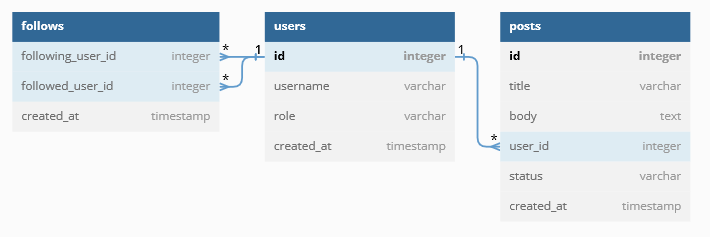
\includegraphics[scale= 0.8]{dbdiagram}
	\caption{Sample database visualising from: \url{https://dbdiagram.io/home}}
	\label{fig:dbdiagram}
\end{figure}

\subsection{Suggestion of Structure Faults}

After the SQL has been parsed and the database has been displayed to the user, the application should provide advice and possible faults of the database, if there are any. This should be clear and direct, and it also should provide feedback as to how to fix this issue. This would involve an analysis of the database structure to see if there are any keys missing or an incorrect design of the database.

\subsection{Scope}

Another goal for this project was to create parsing for the DQL (Data Query Language). This would involve allowing the user to not only input their table structure but also their entries in the tables. This would allow the user to enter a query for the database, and this project would be able to parse the query and return the result of the query to the user. The user would then test for themselves to see if the returned entries were what they expected from their queries. However, this proved to be extra features that were not needed for the scope of this project, as it only mentioned identifying database design flaws and would prove to take too much time than the project allows.

%Include the auto-fixing of the database structure?

\section{Requirements}

\begin{center}
	\captionof{table}{\label{fig:fr}Functional Requirement Table}
	\setlength\extrarowheight{2pt}
	\begin{tabularx}{\textwidth}{|X|X|X|}
		
		\hline
		\textbf{Functional Requirement Number} & \textbf{Functional Requirement Name} & \textbf{Functional Requirement Description} \\
		\hline
		FR-1 & Validate SQL & The user can input text and have syntax highlighting \\
		\hline
	\end{tabularx}
	
\end{center}

\newpage

\section{Process}

For this project, a process adapted from Scrumban was used. The elements of Scrum that were incorporated were:  
\begin{itemize}
	\item Week-long sprints with weekly review and retrospective sessions for iterative planning at regular intervals.
	\item These meetings dictated how much work was pulled into the sprint based on complexity and priority of the work.
	\item Assured necessary levels of analysis and design before starting development.
\end{itemize}
The elements of Kanban that were incorporated were:
\begin{itemize}
	\item In addition to the weekly review and retrospective sessions, a short time was dedicated to process improvement.
	\item Kanban board to provide visualisation of the current items that were in progress, To-Do or in the Sprint Backlog.
	
	\begin{figure}[h!]
		\centering
		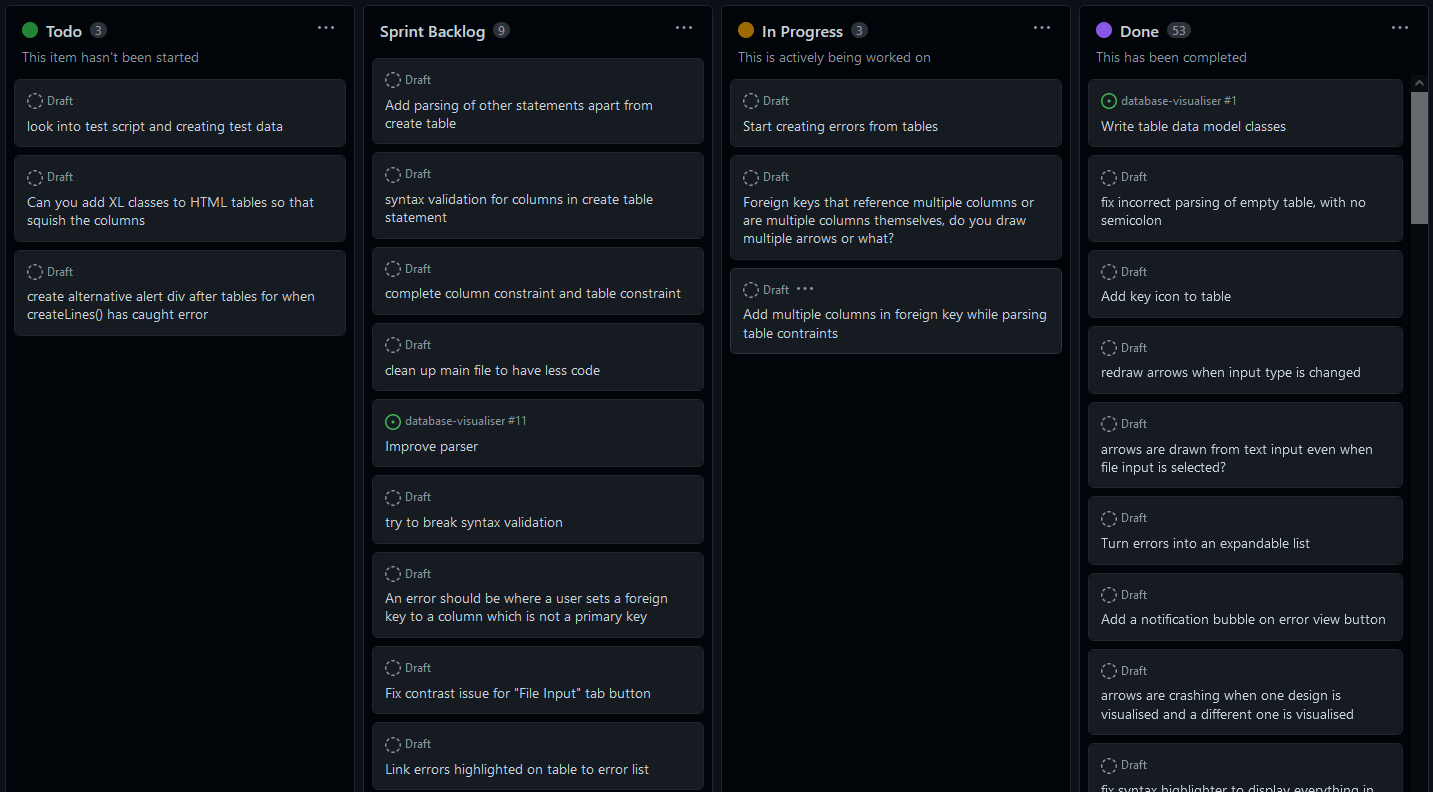
\includegraphics[width=\textwidth]{kanban}
		\caption{Kanban board used for the process of the project.}
		\label{fig:kanban}
	\end{figure}
\end{itemize}

%\addcontentsline{toc}{chapter}{Development Process}
\chapter{Design}

\section{Overall Architecture}

The overall architecture of the project consists of a dynamic webpage with scripting to process user SQL and display back the database structure. The webpage has an input form for the user to enter the SQL as either a file or text. From there, the SQL code is parsed by the JavaScript functions. 

The application attempts to build a database from the user input and if it succeeds it will display the database as a collection of tables on the webpage. If the system fails to build the database it means that the SQL entered has some syntax errors and can not be visualised. Once the database has been visualised, the user can interact with the database by viewing the syntax highlighting of the SQL text, as well as the list of flaws of the database.

\subsection{Consideration of Other Designs}

During the research stage of the project the aim was to find a third-party library that would handle SQL parsing, this will allow the project to focus more on the visualising and structuring of the output. However this proved to not be possible since there were no open-source libraries available to parse the SQL and create an object that could be used to visualise the parsed database. Since this was not possible the main goal of this project was to create an SQL parser that would be able to check if the SQL compiles and if it contained any syntax errors.

Another design that was considered comprised of assuming that the user inserted SQL that compiles and had no syntax errors, an example of this could be an exported file from a database management system. This would make parsing easier since syntax error detection would not have to be implemented, instead, the parser could include more syntax from the documentation and more time could be allocated to detection of more sophisticated database flaws like normalisation. However, the decision was made to instead focus on syntax error detection and include it in the parser since this project is aimed at SQL learners, this means they are more likely to enter SQL with syntax errors which has to be addressed.

\section{Code Structure}

The code is structured into classes that follow the data model of a database, this structure uses an object orientated approach using JavaScript ES6 classes. The classes are closely related to the properties of the PostgreSQL database, this means that a created database object will contains schemas, tables and columns just like a PostgreSQL database. This approach was taken to be able to create a "database" object and from there be able to visualise that object, which improves readability of the code base. 

The syntax errors in the SQL are also implemented in the JavaScript code as an error that are thrown when the database object could not be created due to syntax errors in the SQL input. This allows the creation of alerts to inform the user of the syntax error, the error message is displayed to the user in the alert.
% elaborate more on the syntax error alerts

\newpage

\subsection{Class Diagram}

\begin{figure}[h!]
	\centering
	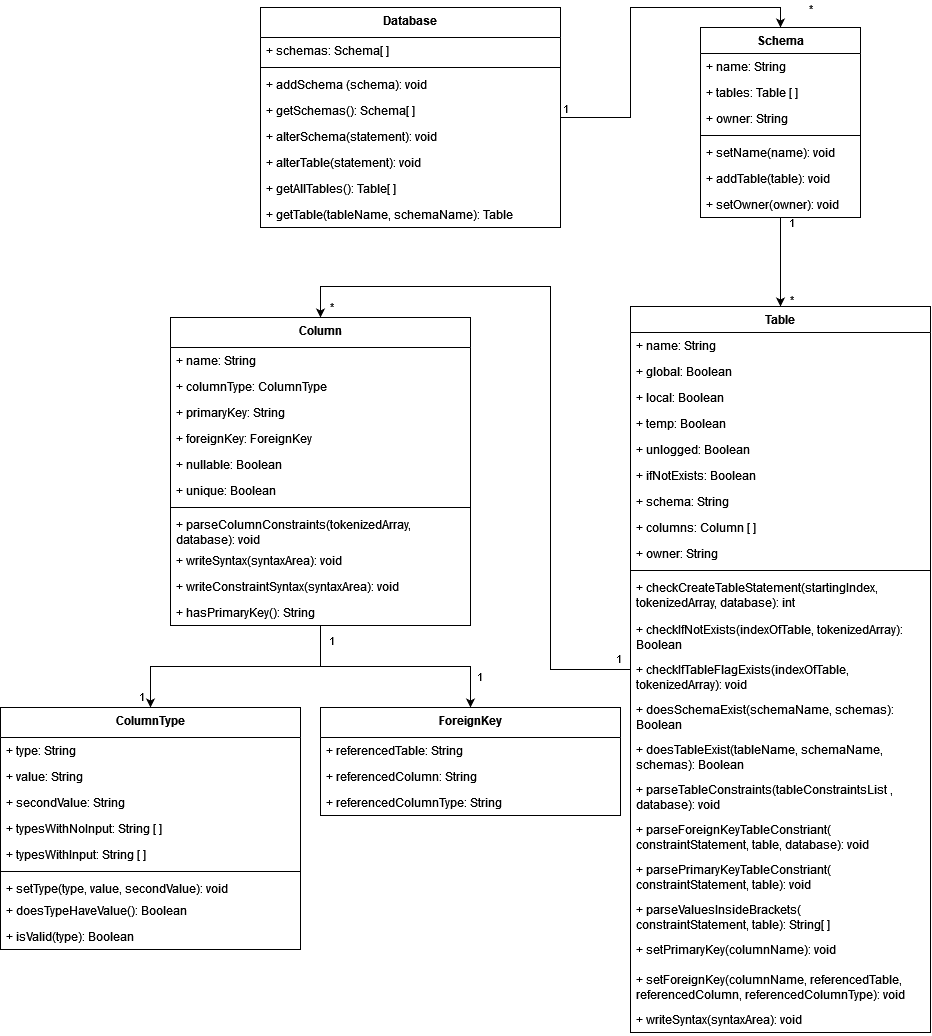
\includegraphics[width=\textwidth]{classDiagram}
	\caption{UML Class diagram for the project, created using diagrams.net\cite{dbdiagram}.}
	\label{fig:classDiagram}
\end{figure}

\newpage

\section{Algorithms}

\subsection{Parser}

As mentioned in the first chapter, the parser consists of a tokeniser and the proper parser. To tokenise the input text, a library was used called js-tokens\cite{tokeniser}. It is designed to tokenise JavaScript code however, for the purpose of parsing SQL it is also appropriate. 

This library is powered by regular expressions and it almost complies with parsing specification. It was chosen because the token object it creates are easy to work with and the types of tokens are compatible for the parsing of the SQL. The library consisted of a function that converted a string into token objects that were later converted into an array. 

The Token objects contained the type of token it was, as well as the value of the token. This made parsing easier since after tokenising the input text, all white spaces could be ignored easily. That left tokens that would either be of type "Punctuator" or "IdentifierName", "Punctuator" tokens would only contain punctuation and "IdentifierName" tokens contained words with numbers. 

This meant that the array of values to parse only contained words which were separated by punctuation. These values could easily be parsed to identify the syntax of each statement by checking against the SQL syntax patterns.

\begin{figure}[h!]
	\centering
	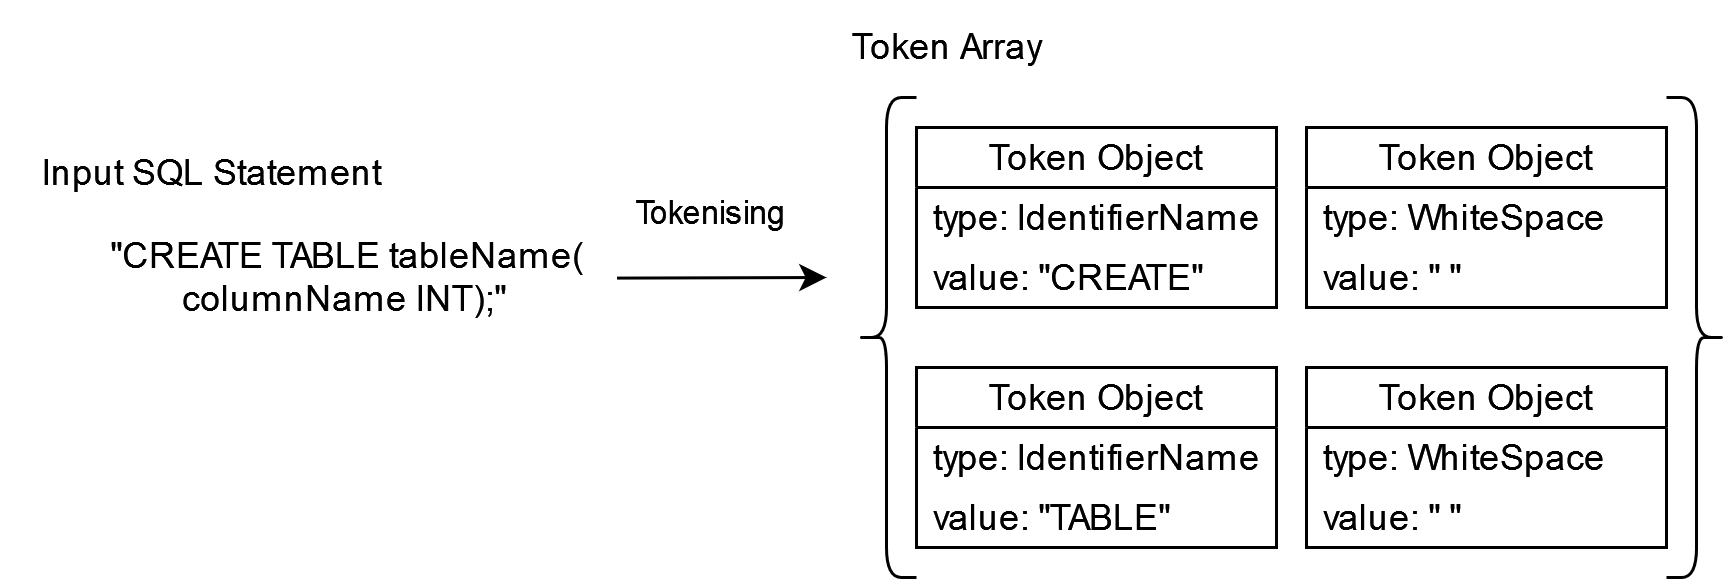
\includegraphics[width = \textwidth]{tokenisingDiagram}
	\caption{Diagram visualising the tokenisation process in the parser function, created using diagrams.net \cite{dbdiagram}.}
	\label{fig:tokenisingDiagram}
\end{figure}

After the input has been tokenised, the proper parsing has to be done analyse the SQL and check if there are syntax errors. This is achieved using regular expressions and further proper parsing. The regular expressions were created to match simple patterns in the SQL syntax, an example of this includes separating each SQL statement by a semicolon. Another example of this is separating each column in a "CREATE TABLE" statement. 

Each column should be separated by a comma, however commas are also present when a primary key is created with more than one column. To achieve this a regular expression was constructed to use Lookahead and Lookbehind, this was used to see if the comma is surrounded by brackets and if it was that comma was not matched.

\begin{figure}[h!]
	\centering
	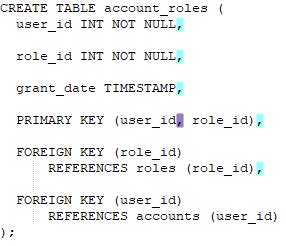
\includegraphics{regex}
	\caption{Comma highlighted in purple is the comma that is missed out from the matching using the regular expression to separate each section of syntax in the "CREATE TABLE" SQL statement.}
	\label{fig:regex}
\end{figure}

Regular expressions were also used to sanitize the input data, this included removing lines that were commented in SQL and also removing line breaks. The regular expression that was used to remove line breaks did so regardless of operating system that used to write the input text. This was done before the input string was tokenised which meant that less sanitizing of tokens had to be done later on in the parser functions.

The other part of parsing consists of going through the split up statements and checking the type of statement that it is, and to examine if the syntax matches the PostgreSQL documentation.  This was done by iterating through the array of token objects and matching the value against a dictionary of words that corresponded to the SQL syntax. 

Depending on the value of the token a different constructor was called to create the corresponding object and add it to the database. The dictionary look-up approach was also taken when checking if a data type of a column in a table is valid. The value of the token that is the data type is checked against a dictionary of possible data types that are available in PostgreSQL.

\subsection{Creating Tree Structure}

The main algorithms involve converting the database object into a tree structure of tables that are then visualised. This is done after the SQL has been parsed and the database object is created, all the foreign keys from the database are collected and are converted into key-value pairs. 

The key is set to the table that the foreign key references and the value is set to the table where the foreign key is present, these become the id and parentId of a node. Duplicates are removed to prevent tables from being visualised more than once and roots are determined from this list of keys. 

This is done by finding the tables that have no foreign keys being referenced by them, the roots will determine the root nodes of the tree structure. If there is only one root that means that all the tables entered are joined together by foreign keys, however if there are more roots that means that there are multiple trees of tables that have to be extracted from the list of tables. 

\subsection{Extraction of Trees from list of values}

For all of the roots a tree is created from the list of key value pairs, after each one is created, it's values are removed from the list. The remaining values from this list are used to build the remaining trees of tables. 

This is achieved using a recursive function, given a root key-value pair and the list of key-value pairs it will recursively get all of the values that belong to that pair. This essentially gets all of the members of a subtree given a root node, and from this list a tree structure can be created. 

The worst case big-O runtime for this recursive function is O(N) with N being the size of the tree. Since the size of the tree will not be large due to the database of a learner will most likely not contain many tables it's not a issue and does not need to be optimised further.

\subsection{Building trees from list of key value pairs}

The array of key-value pairs can be formatted into a tree structure by using JavaScript's object references without recursion.  This function was taken from an article \cite{reference} and it iterates through the array of values and creates a reference from each child to its parent and returns the root value which is a pair that has no reference to a parent. The run time of this function is also O(n) with n being the size of the data array. This is achieved by growing an array of children references and since it is done by reference the parents are not accessed or altered in any way.

\begin{lstlisting}[style=JavaScript, caption={JavaScript function to build a tree from a list of key value pairs.}]
function createTree(data) {
	const idMapping = data.reduce((acc, el, i) => {
		acc[el.id] = i;
		return acc;
	}, {});
	
	let root;
	data.forEach(el => {
		// Handle the root element
		if (el.parentId === null) {
			root = el;
			return;
		}
		// Use our mapping to locate the parent element in our array
		const parentEl = data[idMapping[el.parentId]];
		// Add our current el to its parent's `children` array
		parentEl.children = [...(parentEl.children || []), el];
	});
	return root
}
\end{lstlisting}

\subsection{Drawing HTML Tables as a tree}

If there are foreign keys present in a database, the tables that are linked by those foreign keys are visualised on the webpage as a tree node structure. This is laid out on the webpage using HTML lists. These HTML lists are also structured in a tree node structure, this means that the tables have to be created in the order of left to right. This is the equivalent to depth-first exploration of a tree which is how this was programmed. 

The drawing is done by a function that recursively iterates through the tree depth-first, and depending if the node is a leaf or branch it will either create a HTML list item or an unordered list. This is determined by checking if the current done has children or not and if it does create a new list and draw all of the children of the current node in that list. 

The tables are drawn in HTML lists because CSS styling is used to position the list items in the list horizontally like a tree node diagram is normally visualised. HTML lists were used since they naturally follow a tree structure so it was simple to adapt this structure to draw HTML elements like tables in a tree node diagram structure. 
% if this is hard to understand create a diagram to show the comparsion between HTML structure and table structure

 \begin{lstlisting}[style=JavaScript, caption={JavaScript function that draws a list of tables recursively in HTML list elements.}]
 function drawTreeTablesRecursively(tree, appendNode, tables) {
 	var item = document.createElement("li")
 	for (const table of tables) {
 		if (table.name == tree.id) {
 			table.createTable(item)
 		}
 	}
 	appendNode.appendChild(item)
 	if (tree.children == undefined) {
 		return
 	} else {
 		var list = document.createElement("ul")
 		item.appendChild(list)
 		for (const childNode of tree.children) {
 			drawTreeTablesRecursively(childNode, list, tables)
 		}
 	}
 }
\end{lstlisting}

\section{Data Structures}

The data structures that were used in this project were mostly comprised of arrays of objects and tree node structures. The database classes mostly contained the arrays of objects, while the algorithm that was used to draw the tables used the tree node structures and a list of key-value pairs. In the parsing of the SQL code the tokenising library \cite{tokeniser} created an array of token objects as an output which was the main data structure of the parsing algorithm.

\subsection{Tokenised Array}

The tokenised array is an array of token objects and each token object consists of a type and value, these arrays of tokens are created from the SQL statement string. The token type specifies the type of value which the token has, there are many types which are used for parsing JavaScript code. This array of tokens is a core element of the parsing algorithm that is used in this project.

 \begin{lstlisting}[style=JavaScript, caption={Tokenised array of tokens from a part of a simple input of an "CREATE TABLE" statement.}]
	{ type: "IdentifierName", value: "CREATE" },
	{ type: "WhiteSpace", value: " " },
	{ type: "IdentifierName", value: "TABLE" },
	{ type: "WhiteSpace", value: " " },
	{ type: "IdentifierName", value: "account_roles" }
\end{lstlisting}

\subsection{Key-Value Pairs}

The key-value pairs that represent the foreign keys are stored as an array of objects with pair values. The key and values are stored as id and parentId in each object.

 \begin{lstlisting}[style=JavaScript, caption={Representation of the array of objects containing the key-value pairs.}]
	{ id: "accounts", parentId: "account_roles" },
	{ id: "roles", parentId: "account_roles" },
	{ id: "account_roles", parentId: null }
\end{lstlisting}

For the root pair it has no parent node, therefore to represent that it's parentId is set to be null. This is fairly common practice to store this data for a one-to-many tree node relationship.

\subsection{Tree Node Object}

The tree node object is a an object that has a key and a value in the form of the id and parentId and a list of children with each of them having their key-value pairs and more children nodes. This is a one-to-many relationship so there can be many children to each node.

 \begin{lstlisting}[style=JavaScript, caption={}]
 	Object {id: "account_roles", parentId: null, children: (2) {
 		0: Object { id: "accounts", parentId: "account_roles" },
 		1: Object { id: "roles", parentId: "account_roles" }}
 	}
\end{lstlisting}

\newpage

\section{User Interface}

The user interface was designed so it was simple and easy to use since it was aimed at SQL learners. It was designed to be used on a desktop computer with a medium to large monitor. The core of the design has been the same throughout the project, however some of the elements have undergone major changes to the styling or layout. It was designed using Bootstrap 5 \cite{Bootstrap} which is a front-end toolkit, it was used to do all of the styling and for the key icons. It was used to give the website a more professional and uniform look, after the colour scheme was chosen and entered, bootstrap modified all elements to follow this colour scheme.

There are two main elements to the user interface: 

\begin{itemize}
	\item \textbf{The Input Form} - The input form is how the user enters their SQL database design into the website for the script to process it. It has two tabs: "Text Input" and "File Input". These can be chosen to either enter text into the text area or upload a file into the file picker.
	\item \textbf{The Visualised Views} - Once the SQL has been validated, the "Visualise" button can be pressed and the visualised database view tabs appear. These tabs include: "Table View", "Syntax View" and "Problem View". Each of these is a separate page that contains information or a visualisation of the entered SQL database.
\end{itemize}

\begin{figure}[h!]
	\centering
	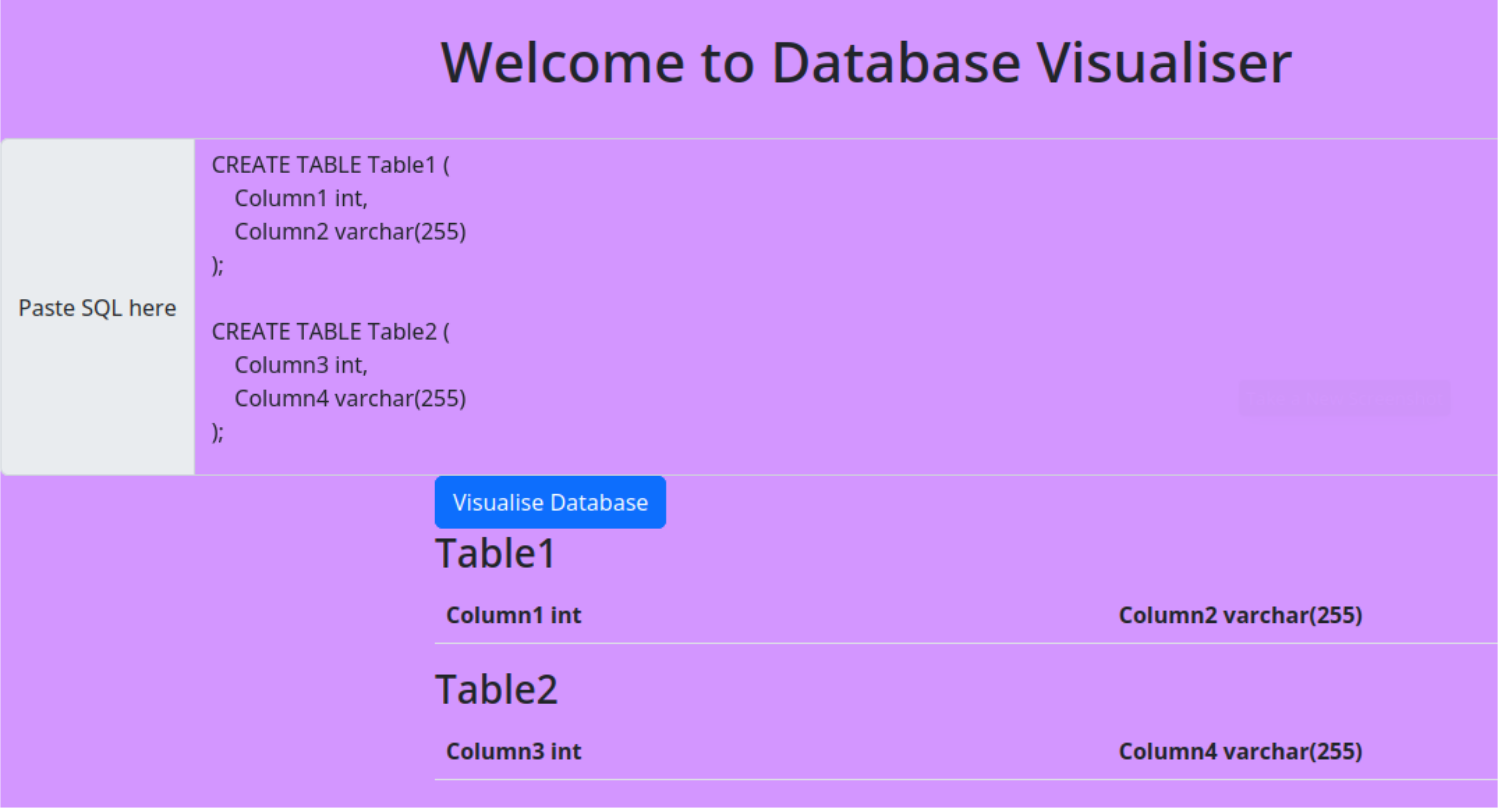
\includegraphics[width=\textwidth]{firstDesign}
	\caption{First iteration of the user interface design.}
	\label{fig:firstDesign}
\end{figure}

The first iteration of the design included the input form with the only option of input being text with crude parsing of the SQL. The tables are also stretched across the page without borders and styling. The tables here were made using HTML tables however they have the SQL column name and data type as columns in the table which might be confusing, due to this the structure of the tables were changed in the future iterations.

\newpage

\begin{figure}[h!]
	\centering
	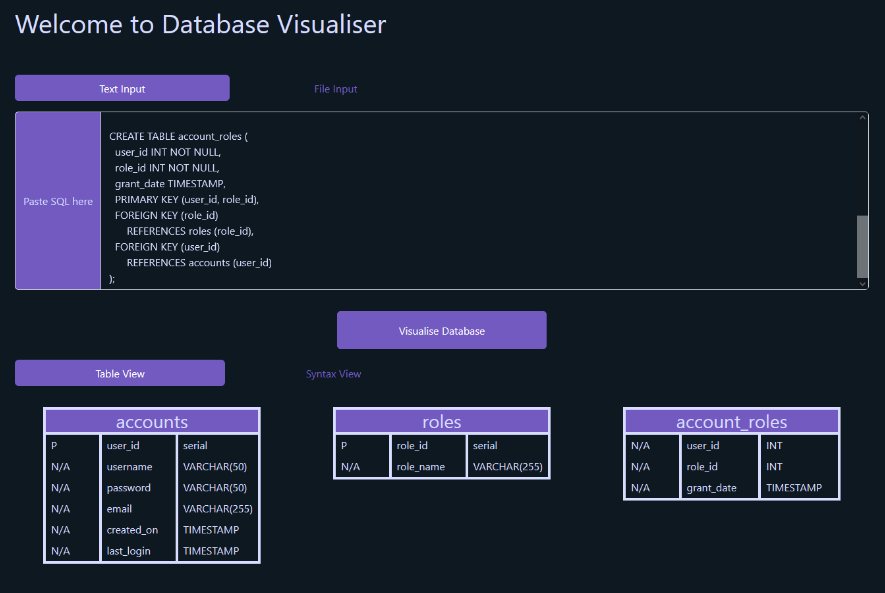
\includegraphics[width=\textwidth]{secondDesign}
	\caption{Second iteration of the user interface design.}
	\label{fig:secondDesign}
\end{figure}

The second iteration of the design had a much better colour scheme following the website trend of having a dark background with white text and lighter accent colours. It now also includes the option to change the input form from text to file input, as well as the output tabs being created below the visualise button for the table output and syntax highlighting output. 

However the foreign key arrows have not been implemented yet and the tables here are visualised in the order that they are created in the SQL file. Also the primary key icons are also not yet added and instead are represented as either a "P" for being part of a primary key constraint and "N/A" for not being part of a primary key constraint.

\newpage

\begin{figure}[h!]
	\centering
	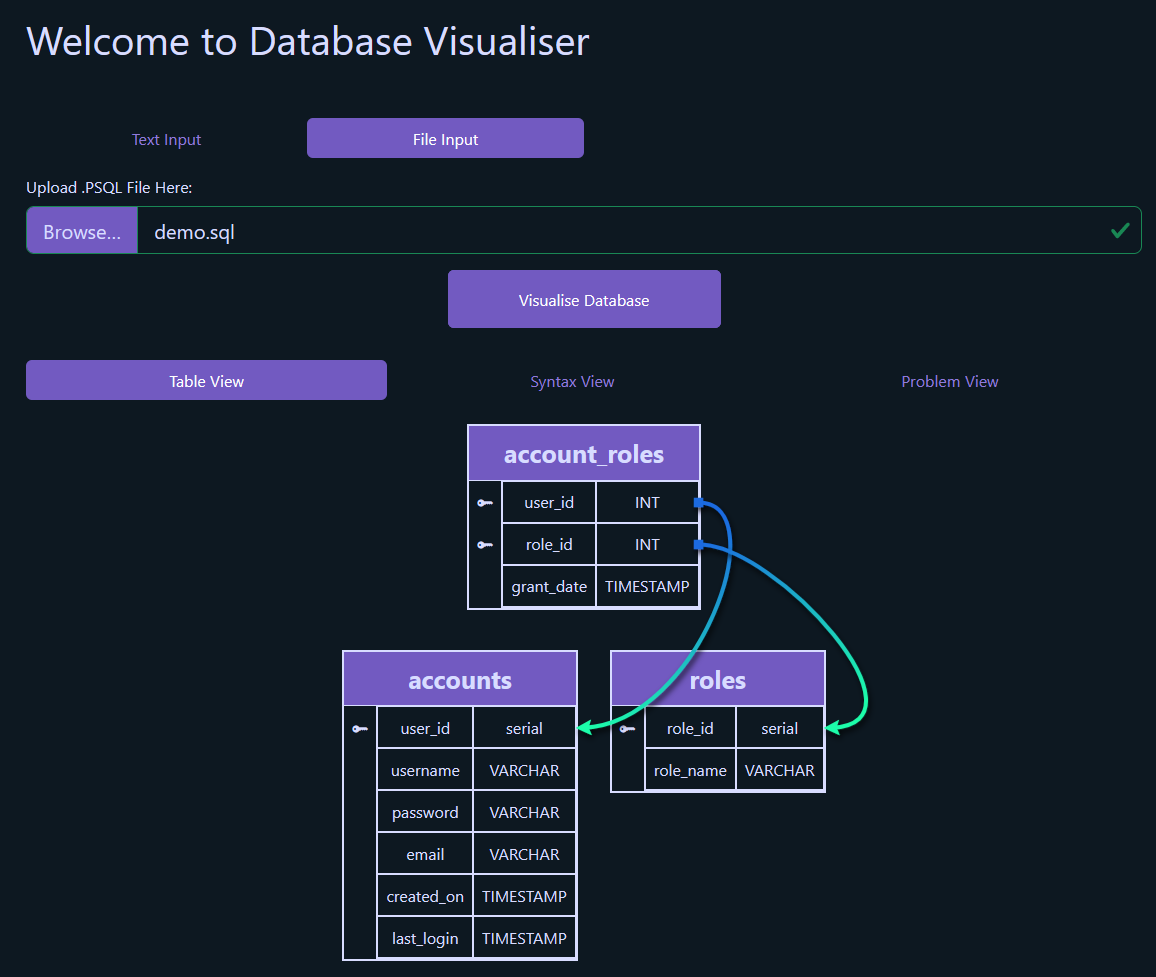
\includegraphics[width=\textwidth]{finalDesign}
	\caption{Final iteration of the user interface design}
	\label{fig:finalDesign}
\end{figure}

The final design builds from the second iteration by adding the tree node structure layout to tables and the foreign key links between them. The tables are now HTML tables and not the Bootstrap tables made out of row and columns div elements which makes them look slightly more compact and more professional. There are now key icons for the primary key column in each table for the columns that are part of the primary key constraint. It also includes the green outline and tick icon for the input form that is shown when the SQL in the input file, is valid and compiles. The colour scheme has stayed the same since it has not interfered with any of the other elements and did not need to be changed. 
\chapter{Implementation}

\section{Issues Encountered During Implementation}

\subsection{Creating tables using bootstrap}

Initially it was decided to create the SQL tables during visualisation using the Bootstrap 5 Grid system. Using a series of rows and column in a flexbox it can layout and align the content dynamically. This seemed like a good tool for creating tables because it allowed for creation of custom layouts for tables and it would give more freedom for styling and highlighting since it is not a restrictive structure of a HTML table element. This was the reason that HTML tables were not used for this because the table cells will be empty since the SQL parsing will not be done for "INSERT" statements so no entries will be added to the tables.

Later on in the implementation of this tables when the parsing was sophisticated enough to parse large tables, the problem emerged of Bootstrap shifting the layout of the tables and squashing it's columns together to look like rows on smaller screen or if the window was resized. The grid system is useful when building layouts for mobile-first designs and the changing the layout when the screen size is smaller is useful, but not for this project since learners are not going to be writing their sql databases on a mobile device. 

\begin{figure}[h!]
	\centering
	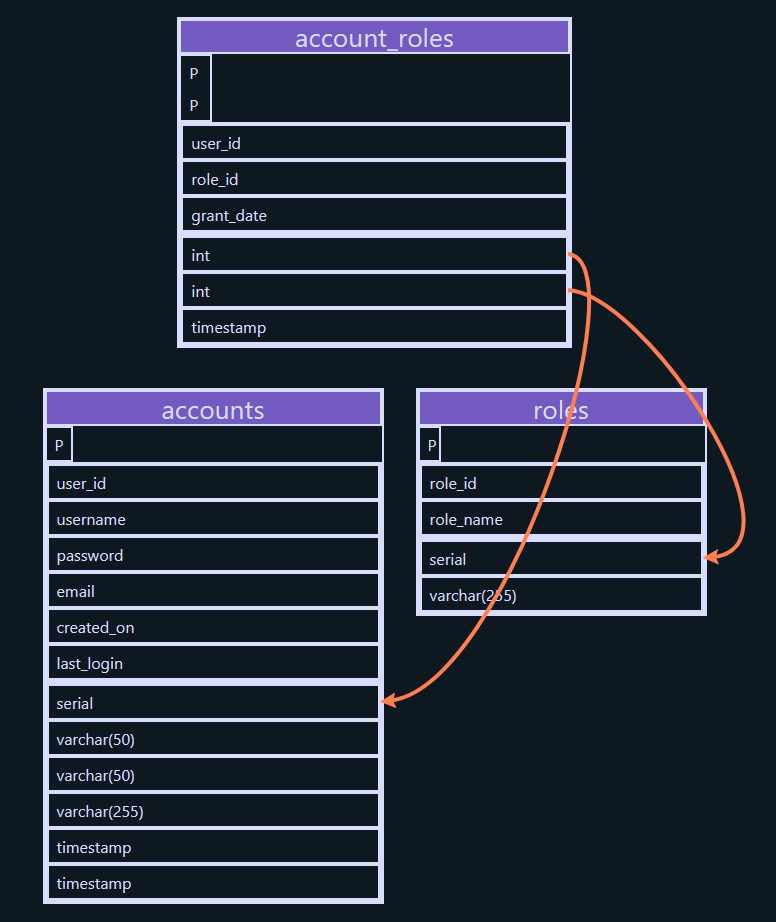
\includegraphics[scale=0.5]{postSquash}
	\caption{Visualisation of tables showing the column being compressed to look like rows in a single column due to the flexbox responsive resizing.}
	\label{fig:squash}
\end{figure}

This problem was solved by going back to using HTML table elements and dynamically creating tables from the table objects. This solution was slightly harder to implement however the and layout was much better since Bootstrap did not resize the table element. This was because the entire table is viewed as an element which prevents it from being changed when the window is resized, compared to the previous implementation which had a single column be an element which was resized. Bootstrap provides styling classes for tables which made the styling easy to change as it was before using the previous tables.

\begin{figure}[h!]
	\centering
	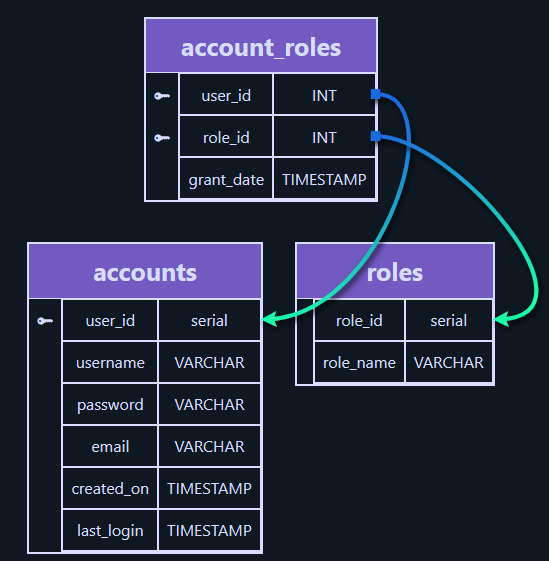
\includegraphics[scale=0.7]{newPostSquash}
	\caption{Visualisation of tables after a structure using HTML table elements was adopted, showing no signs of distortion after changing the size of the window.}
	\label{fig:afterSquash}
\end{figure}

\subsection{Early stages of parsing}

Early stages of parsing used simple checking of strings and struggled separating spaces properly, as well as punctuation and created complex regular expressions that were hard to read and were prone to break. Used the tokenising library that made it easier to create some data structure that was easy to work with and made the parsing a lot easier. Parsing was a lot more complex than initially thought. Lot's of edge cases for SQL and an immense complexity in the number of possible statements and combination of statements. Lot of work went into implementing parsing for just a few statements however, this just took a longer time to write than expected but it was done.

\subsection{Drawing arrows library}

Drawing lines between two HTML elements was something that had to be done to represent foreign key relationships between tables. One possible way to do was to use a HTML canvas and draw lines using the elements positions. However this was difficult to style correctly to match the design and would require more work to create a function to do what is required. Instead, a library leader-line \cite{leader-line} was used to draw an arrow between two elements. The styling of this arrows was much easier to do and it also included some implementation for animations which made the design look much better.

\subsection{Drawing Tables on the webpage}

Drawing the tables in a way that was easy to understand was difficult because the order or layout the tables are displayed in plays a key role in how easy a database can be understood. It was first implemented to display the tables in the order in which the tables appeared in the SQL text file since it seemed logical to do so because the learners will expect the tables to be displayed in this order. However once foreign key arrows were implemented then the tables had foreign key constraint arrows across them because the tables that were joined together were not together in the sql text file. This was quite confusing to try to understand and a decision was made to display them in a more organised structure. 

\begin{figure}[h!]
	\centering
	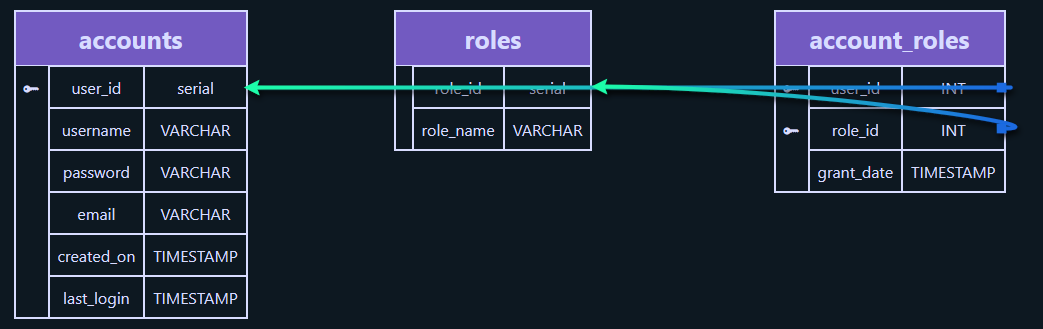
\includegraphics[width=\textwidth]{overlap}
	\caption{Visualisation of tables in the order of creation with drawing of arrows depicting overlap between the tables and arrows prevent text in columns to be readable.}
	\label{fig:overlap}
\end{figure}

\subsection{Implementing Highlighting of Text in a HTML TextArea}

The HTML Textarea is what is used in the website form to enter the SQL text by the user, to be user-friendly, if the entered SQL has some syntax errors it should highlight roughly where the error is. This is important because an SQL learner will not be able to easily spot where their error is in the SQL, since they are not familiar with the syntax. 

\begin{figure}[h!]
	\centering
	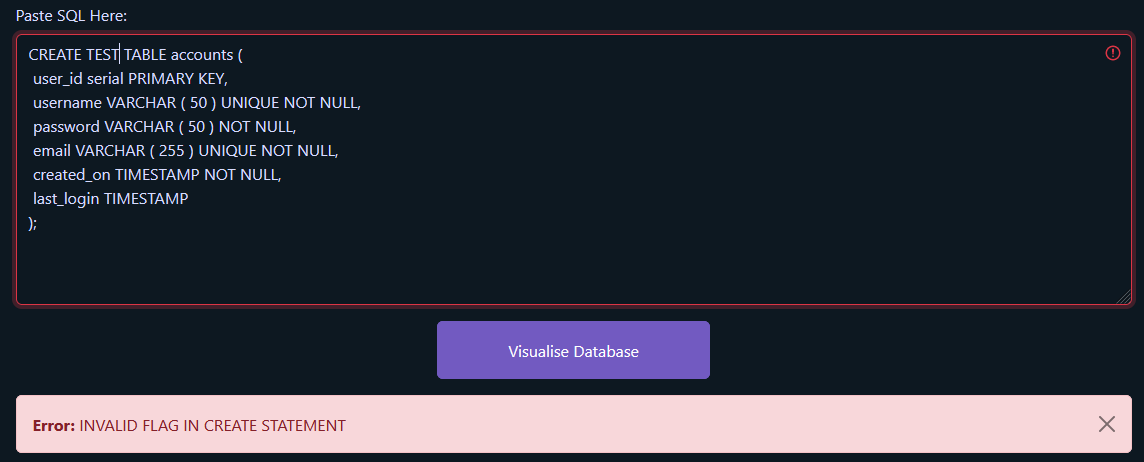
\includegraphics[width=\textwidth]{textArea}
	\caption{Initial implementation of the textArea validation and syntax error alert.}
	\label{fig:textArea}
\end{figure}

The HTML Textarea does not natively have the functionality to highlight text inside of it, any mark up to the text would appear as plain text. A possible solution to this problem is to implement a rich text editor in the webpage and replace the Textarea with it, rich text areas can provide implementation to highlight and mark up text much better and easier than the Textarea. However building a rich text editor is not the easiest to do since even basic functionality is difficult to implement \cite{highlightText}.

However since adding a already functioning text editor to the webpage would require styling it and cutting down all of the features down only to the highlighting, it was decided to create a work around for the Textarea. This was done by creating a "fake" textarea under the current one that only looked like a textarea and since it was overlayed over the textarea, it was not perceivable by the user. The goal of this textArea is to only highlight the text and since it is a div that looks like a textArea this can be done by creating span elements of the words that have to be highlighted that had some styling. This proved to be quite easy to implement and provides the solution to the problem.

\begin{figure}[h!]
	\centering
	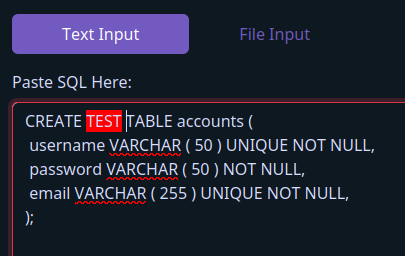
\includegraphics[scale = 1]{highlightedTextArea}
	\caption{Later implementation of the highlighting of the origin of the syntax error in the input textarea.}
	\label{fig:highlightedTextArea}
\end{figure}

\newpage

\section{Review of Requirements}

The initial requirements are all mostly met apart from the functionality that is outside the scope of this project that is mentioned previously in the report. 

\begin{center}
	\captionof{table}{\label{fig:reviewOfImplementation}Table reviewing the initial table of requirements}
	\setlength\extrarowheight{2pt}
	\begin{tabularx}{\textwidth}{|X|X|X|}
		\hline
		\textbf{Functional Requirement Number} & \textbf{Functional Requirement Name} & \textbf{Review of Requirement} \\
		\hline
		FR-1 &  Enter SQL into website form & The user can enter their SQL in either text form in the textarea or in file form by uploading their file into the filepicker. The website processes the correct data that the user provides. \\
		\hline
		FR-2 & Validate entered SQL & Once the data has been entered the SQL is validated and feedback is given to the user through the styling of the form and the alerts whether the SQL is correct or has syntax errors. \\
		\hline
		FR-3 & Visualise entered database & The entered database is visualised by creating tables and the links between them.\\
		\hline
		FR-4 & View highlighted syntax after visualising & Once the database has been visualised, the "syntax view" tab can be selected to find the highlighted and indented SQL that had been entered before. \\
		\hline
		FR-5 & The user can filter through data types of columns in syntax view & At the syntax view tab there are filters that can be checked to highlight the data types to a green colour to separate them from the rest. \\
		\hline
		FR-6 & The user can view the flaws of the database & Once the database has been visualised, the "Problem View" tab can be selected with a list of flaws that the database might have, if there are no flaws detected then the user is prompted with a message. \\
		\hline
	\end{tabularx}
\end{center}
\chapter{Testing}

\section{Overall Approach to Testing}

The overall approach used to testing was a combination of both automated and manual testing. Unit tests were written for the parsing algorithm of the project and manual testing was done for integration testing. The testing should show that the project can take in some SQL from a user and subsequently parse and visualise it in a way to make it simpler for the user to understand SQL. Unit testing the parsing algorithm shows that the validating is working correctly and catching the correct syntax errors with the entered SQL. Manual testing is used to test the entire system working together and making sure that the initial requirements are met and the user can use the system without problem and can get some use out of it.

\section{Automated Testing}

The automated testing addresses the requirement of validating the entered SQL. The parsing algorithm was written to be testable by throwing an error if the SQL does not validate. The unit tests can then catch that error and check that the error message to the user is correct and the parser is throwing the correct error. The unit tests were written using a testing framework for JavaScript called Mocha\cite{mocha}. The unit tests are written to test parsing either just a string of a SQL statement or an entire file of an SQL database dump file containing an entire database. Testing an entire file tests that an entire database can be parsed and correctly find that no errors are present. Testing simple statements that are missing parts of the syntax tests that the parser is detecting the correct syntax errors in the SQL and is giving the user correct feedback. The unit test are also testing the behaviour if data is entered that is meant to break the system which tests for the robustness of the parser.

\subsection{Unit Testing Test Table}

\begin{center}
	\captionof{table}{\label{fig:unitTestTable}Table showing examples of the unit tests that were written, all of the following tests reference the SQL validation requirement (FR-2).}
	\setlength\extrarowheight{2pt}
	\begin{tabularx}{\textwidth}{|c|X|X|X|c|}
		\hline
		\textbf{Test ID} & \textbf{Description} & \textbf{Input} & \textbf{Expected Result} & \textbf{Pass/Fail} \\
		\hline
		ATC-1 & Parser should throw syntax error & Validate the statement: "CREATE TABLE" & Error should be thrown with the message "Missing Semicolon in statement" & Pass \\
		\hline
		ATC-2 & Parser should not throw a syntax error & Validate the test.sql file & Validation should be complete without syntax errors being thrown & Pass \\
		\hline
	\end{tabularx}
\end{center}

\section{Manual Testing}

Manual testing was done because the system is quite complex to test using a testing framework. This part of testing tests the entire system and follows the steps that the user might follow but also steps that could potentially break the system. The manual testing was done to make sure that the requirements have been met that are not to do with the parsing since that was covered by the unit tests, parsing is involved in these tests however what is being tested is that the system as a whole reacts correctly to the output of the parsing and also that the output matches for the same case as the unit tests. This is done to test that the parsing works correctly when it is isolated in unit tests but also when it is part of a much larger system.

\subsection{Manual Testing Test Table}

\begin{center}
	\captionof{table}{\label{fig:manualTestTable}Test table listing the manual tests.}
	\setlength\extrarowheight{2pt}
	\begin{tabularx}{\textwidth}{|c|c|X|X|X|c|}
		\hline
		\textbf{Test ID} & \textbf{Reference} & \textbf{Description} & \textbf{Steps} & \textbf{Expected Result} & \textbf{Pass/Fail} \\
		\hline
		MTC-1 & FR-1.1 & Entering valid SQL into the textarea & Enter a valid SQL statement into the labelled text area. & Text area border should turn to a green colour and the "Visualise" button should be enabled & Pass \\
		\hline
		MTC-2 & FR-1.1 & Entering invalid SQL into the textarea & Enter an invalid SQL statement into the labelled text area. & Text area border colour should turn to a red colour and an alert should appear with the syntax error & Pass \\
		\hline
		MTC-3 & FR-1.2 & Entering an valid SQL file into the filepicker & Enter an valid SQL file into the filepicker. & Text area border should turn to a green colour and the "Visualise" button should be enabled & Pass \\
		\hline
		MTC-4 & FR-1.2 & Entering an invalid file into the filepicker & Enter an invalid SQL file into the filepicker. & Filepicker border should turn to a red colour and an alert should appear with a message that the filename is invalid. & Pass \\
		\hline
		MTC-5 & FR-3 & Visualising a test database from file & Upload the file test.sql into the filepicker and press the "Visualise" button. & Test database should be visualised correctly with the foreign key arrows. & Pass \\
		\hline
		MTC-6 & FR-4 & Viewing the syntax highlighting & Upload the file test.sql into the filepicker and press the "Visualise" button, then press the "Syntax View" tab button. & Syntax highlighting of the test database should be displayed with correct colours, syntax and indentation & Pass \\
		\hline
		MTC-7 & FR-5 & Using the filters in syntax view & Upload the file test.sql into the filepicker and press the "Visualise" button, then press the "Syntax View" tab button and press the "serial" checkbox . & All of the "serial" data types should be highlighted in a green colour. & Pass \\
		\hline
		MTC-8 & FR-6 & View a database flaw & Upload the file test1.sql into the filepicker and press the "Visualise" button, then press the "Problem view" tab button and press the accordion button. & There should be an user interface element displaying the missing primary key constraint. & Pass \\
		\hline
		MTC-9 & FR-6 & View problems of a database with no flaws & Upload the file test1.sql into the filepicker and press the "Visualise" button, then press the "Problem view" tab button & There should be a prompt for the user to inform them that there are no database flaws detected & Pass \\
		\hline
	\end{tabularx}
\end{center}

\section{User Testing}


\chapter{Evaluation}

\section{Requirement Fulfilment}

Overall, all of the requirements that were identified at the beginning of the project have been met to a good standard. The website is able to visualise simple databases and if there are any flaws detected it will advise the user on how to fix these issues. Despite the SQL parsing not being as rigorous as expected the validation in the form works and will catch simple syntax errors that the user might make and inform them of it. The website has a simple and intuitive user interface, with minimalistic styling and theme.

\section{Identification of Requirements}

The identification of requirements was reasonable for the length of this project. The goals were set to be challenging yet attainable. As mentioned in the scope of this project \textit{\hyperref[subsec:scope]{Scope}}, parsing Data Query Language and creating an algorithm to automatically repair databases would be outside of the scope of this project. All of the requirements are necessary for this application to be useful to SQL learners.

\section{Evaluation of Methodology Used}

As discussed in \textit{\hyperref[sec:process]{Chapter 1}}, a process adapted from Scrumban was used. The use of this methodology was beneficial because it gave a solid structure to the development of this project. The weekly sprints were useful because planning was done at the beginning of the sprint for what was going to be worked on in that week. This made it easier to focus on a few issues or implementations at a time and the Kanban board allowed the visualisation of issues and their completion stage. During each sprint additional issues were raised as work was being done and were added to the sprint backlog which was reviewed at the end of the week to create a new set of issues to work on during the late weeks. 

However an improvement for this approach to the project would have been focusing more on testing in the beginning stages of development. The testing framework should have been looked into during spike work and test should have been written throughout the development process. A framework for integration testing for the entire website should have also been looked into, it would be useful to be able to automatically test the website as a whole and test the interaction of components.

\section{Were the design decisions correct?}

The design of the project was mostly correct, more thought might have gone into designing a more efficient parsing framework however this would require more time. A more in-depth parsing framework would allow to have more exhaustive parsing and better syntax error feedback to the user with the line number where the error is and maybe a link to the highlighted text.

The decision to use object-orientated JavaScript was a good design decision since it worked well in this application and the code is readable and structured. Inheritance was used to prevent code duplication in some cases and class choices to follow the data model of a database was a good choice since it gave a logical layout to the classes, and gave more context to some of the functions.

The design decisions for the user interface were good because the website is easy to use for SQL learners and conveys the information efficiently and directly. The decision to layout the tables into a tree structure was correct because it was much clearer than laying out the tables in creation order and was appropriate for this application.

\section{Choice of Tools and Development Environment?}

The choice of the development environment was good as there were no issues during the development of the project. The website was developed on a local development server which provided instant feedback on the changes made to either the code or the styling of the website, this was done using Node.js. There were also no issues with lacking functionality from the IDE or the website hosting servers. 

The choice of using native JavaScript was good for the current state of the project. In the future if the parsing framework was expanded and more functionality was added to the website which would require more user interface elements then potentially a JavaScript framework would be more appropriate. One of these frameworks could be React which would allow the creation of reusable components that would need to be created if the website had more features that would require user interface components. This would require more time to implement these reusable components and learning the framework however it would save time in the future by being able to re-use components. 

The choice of using Bootstrap as the front-end toolkit was correct since it allowed the focus of the project to be on the parsing and the visualising of the tables and less on the styling and design of the website. A more appropriate toolkit might be available that does not focus so much on the responsive and mobile-first design however for the current state of the project it is satisfactory. 

\subsection{Familiarity of the Technology Used}

The familiarity with web development was adequate with native HTML, CSS and JavaScript which was useful for the project since time did not need to be used to learn these technologies. 

However Bootstrap was not used before this project and reading and learning had to be done to get used to designing a website using Bootstrap. If some other toolkit was used that was not so focused on responsive design then the re-designing of the tables might have not been needed. This might have also been avoided if there was familiarity with Bootstrap before the start of this project. 

% cite this back to the squished tables.

\section{Lessons Learnt}

If this project would be reworked then the issue of adequate SQL parsing should be addressed. This project should either adapt an already implemented parser from an API and use it to just parse DDL statements, another way to do this is to contribute to a parsing framework that is not fully developed and add functionality to parse DDL statements. After this issue is solved then more interesting features can be worked on and added to this project.

Deeper exploration of different combinations of frameworks could be done to see if it would be useful when building a more complex website application with more content and features. 

% add to this what else was learnt?

\section{Future Work}

If this project were to be worked on in the future, more advanced detection of flaws in the parsed database should be looked into. This could involve possibly detecting if the database has been normalised and if not see if there is a way to prompt the user to do so. Another flaw detection is to see if the table or column name is plural since it is good design to have names be singular, in addition to this it could also check if the correct naming convention is used in names. Another feature that could be implemented is to prompt the user to inform them that a deprecated feature is used, even though it is correct syntax it should be avoided to use deprecated flags.

In addition to more advanced detection of these flaws, there should be some ranking system created to quantify how serious of a flaw is to the integrity of the database. This could involve ranking a missing primary key as a serious flaw that is high risk where as using a deprecated flag is not even a flaw that has to be fixed, it could be a warning to the user.

Finally since this project is also aimed to be used in teaching, in the future there should be functionality for people marking student databases. This would involve being able to upload many SQL files at a time to parse and detect flaws for all of them and output the results in a suitable form. This most likely not be a replacement for marking since the parsing and flaw detection will need to be much more sophisticated for this use case.

\setemptyheader

\nocite{*} % include everything from the bibliography, irrespective of whether it has been referenced.
\addcontentsline{toc}{chapter}{References} % Adds References to contents page
\bibliographystyle{StylesAndReferences/IEEEannot.bst}
\renewcommand{\bibname}{References} 

\bibliography{StylesAndReferences/references} % References file

\pagebreak

% start the appendix - sets up different numbering
\fancypagestyle{plain}{%
%\fancyhf{} % clear all header and footer fields
\fancyhead[L]{Appendix\ \thechapter}
\fancyhead[R]{\leftmark}}

\appendix
\fancyhead[L]{Appendix\ \thechapter}
\fancyhead[R]{\leftmark}
\fancyhead[C]{}
\fancyfoot[C]{\thepage}
\renewcommand{\headrulewidth}{0.4pt}
\renewcommand{\chaptermark}[1]{\markboth{#1}{}}

\fancyhead[L]{Appendix\ \thechapter}
\fancyhead[R]{\leftmark}
\fancyfoot[C]{{\thepage} of \pageref{LastPage}}

% include any appendices here
\chapter{Third-Party Code and Libraries}

If you have made use of any third party code or software libraries, i.e. any code that you have not designed and written yourself, then you must include this appendix. 

As has been said in lectures, it is acceptable and likely that you will make use of third-party code and software libraries. If third party code or libraries are used, your work will build on that to produce notable new work. The key requirement is that we understand what your original work is and what work is based on that of other people. 

Therefore, you need to clearly state what you have used and where the original material can be found. Also, if you have made any changes to the original versions, you must explain what you have changed. 

The following is an example of what you might say. 

Apache POI library - The project has been used to read and write Microsoft Excel files (XLS) as part of the interaction with the client's existing system for processing data. Version 3.10-FINAL was used. The library is open source and it is available from the Apache Software Foundation 
\cite{apache_poi}. The library is released using the Apache License 
\cite{apache_license}. This library was used without modification. 

Include as many declarations as appropriate for your work. The specific wording is less important than the fact that you are declaring the relevant work.

\fancypagestyle{plain}{%
   \fancyhead{} %[C]{Annotated Bibliography}
   \fancyfoot[C]{{\thepage} of \pageref{LastPage}} % except the center
   \renewcommand{\headrulewidth}{0pt}
   \renewcommand{\footrulewidth}{0pt}
}

%TC:endignore

\end{document}
